% ------------------------------------ %
% Copyright (C) 2020 Marvin Strangfeld %
% ------------------------------------ %
\documentclass[conference]{IEEEtran}

\usepackage{cite}
\usepackage{amsmath,amssymb,amsfonts}
\usepackage{algorithmic}
\usepackage{graphicx}
\usepackage{textcomp}
\usepackage{listings}
\usepackage{xcolor}
\usepackage[hidelinks]{hyperref}
\usepackage{cleveref}
\usepackage{float}

% TODO: Correctly align the caption with the listing frame
\usepackage{caption}
\DeclareCaptionFont{white}{\color{white}}
\DeclareCaptionFormat{listing}{\colorbox{darkgray}{\parbox{\dimexpr\linewidth-0.7em\relax}{#1#2#3}}}
\captionsetup[lstlisting]{format=listing,labelfont=white,textfont=white}

\definecolor{codegreen}{rgb}{0,0.6,0}
\definecolor{codegray}{rgb}{0.5,0.5,0.5}
\definecolor{codepurple}{rgb}{0.58,0,0.82}
\definecolor{backcolour}{rgb}{1,1,1}

\lstdefinestyle{mystyle}{
    backgroundcolor=\color{backcolour},
    commentstyle=\color{codegreen},
    keywordstyle=\color{magenta},
    numberstyle=\tiny\color{codegray},
    stringstyle=\color{codepurple},
    basicstyle=\ttfamily\footnotesize,
    breakatwhitespace=false,
    breaklines=true,
    captionpos=t,
    keepspaces=true,
    numbers=left,
    numbersep=5pt,
    showspaces=false,
    showstringspaces=false,
    showtabs=false,
    tabsize=2,
    frame=single,
    xleftmargin=2em,
    framexleftmargin=1.57em,
    framexrightmargin=-0.5em
}

\lstset{style=mystyle}
\renewcommand{\lstlistingname}{Code}
\Crefname{listing}{Code}{Codes}
\crefname{listing}{code}{codes}

\def\BibTeX{{\rm B\kern-.05em{\sc i\kern-.025em b}\kern-.08em
    T\kern-.1667em\lower.7ex\hbox{E}\kern-.125emX}}
\begin{document}

\title{Finding Concurrency Bugs in Production}

\author{\IEEEauthorblockN{Marvin Alexander Strangfeld}
\IEEEauthorblockA{
    \textit{RWTH Aachen University}\\
    marvin.strangfeld@rwth-aachen.de}
}

\maketitle

\begin{abstract}
% TODO: Why in production?
Today's computer architectures rely more and more on parallel computing.
Single core processors were widely replaced by multi-core architectures optimized to run processes and threads concurrently.
To utilize the full performance of the given hardware, programmers need to write their software with a high degree of parallelism.
This introduces the potential for bugs that would not occur in sequential programs due to non-determinism in the order of execution.
Such bugs can be very challenging to fix because they are not easily reproducible.
For this purpose tools and languages have been developed to ease the creation of concurrency-aware programs and to help programmers find concurrency bugs effectively.
This paper will evaluate three different techniques and concrete tool implementations of them, that are available to find, reproduce and fix concurrency bugs from the viewpoint of how usable they are in a production environment.
The requirements for these tools are that they need to be easy to deploy, they should bring only a minimal computational and storage overhead, they should have a high coverage with minimal false-positive reports and they need to enable the developer to quickly find the cause of a bug.
The techniques evaluated are: Dynamic code analysis with the record and replay tool rr and the data race detector ThreadSanitizer.
Concurrency-aware testing with a combined approach of evaluating thread schedules with delta-debugging to automatically pinpoint concurrency bugs.
Static code analysis with the methods of sequentialization and model-checking.
All tools are evaluated for the Go programming language but the concepts are mainly applicable to every other language as well.
\end{abstract}

\begin{IEEEkeywords}
    [Software Engineering]: Software testing and Debugging
    [Computing methodologies]: Concurrent programming languages
\end{IEEEkeywords}


% ------------------------------------ %
% ----------- INTRODUCTION ----------- %
% ------------------------------------ %
\section{Introduction}

\subsection{Heisenbugs}

\begin{quote}
``Everyone knows that debugging is twice as hard as writing a program in the first place. So if you're as clever as you can be when you write it, how will you ever debug it?'' --- Brian W. Kernighan\cite{kernighan1974elements}
\end{quote}

Writing concurrent programs can be very challenging.
Computational work gets distributed among different processes and threads that need to synchronize to be able to speed up execution time on multi-core architectures.
Due to this complexity it is no surprise that bugs that are correlated to concurrency and parallel program execution occur quite often.
These bugs are also the most difficult to debug because they are so complex in their nature and not easy to reproduce.~\cite{tu2019go}
This is because of the non-determinism that is introduced when multiple threads or processes are executed simultaneously.
In contrast to sequential programs that only run on one thread and process, concurrent programs have multiple paths of execution that are executed more or less independently from each other.
The order these threads are executed is determined by the operating system's scheduler.
Because a developer, like the program itself, cannot predict what resources also need processing time on a machine, the concrete schedule has to be handled as non-predictable and therefore as non-deterministic.
But non-deterministic behavior also means that a bug that is only triggered when a certain pattern of thread executions or thread interleavings appear, cannot be reliably reproduced without knowing the schedule it appeared in.

In 1986 Jim Gray introduced the term ``Heisenbug'' for these kind of software failures.
He wrote:

\begin{quote}
``The assertion that most production software bugs are soft -- Heisenbugs that go away when you look at them -- is well known to systems programmers. Bohrbugs, like the Bohr atom, are solid, easily detected by standard techniques, and hence boring. But Heisenbugs may elude a bugcatcher for years of execution. Indeed, the bugcatcher may perturb the situation just enough to make the Heisenbug disappear. This is analogous to the Heisenberg Uncertainty Principle in Physics.''\cite{gray1986computers}
\end{quote}

The complexity and uncertainty of concurrency bugs is also the reason for many studies that examine how these bugs occur and explore different ways on how to detect, fix or even avoid them.~\cite{tu2019go}
Thus, numerous tools and techniques have been developed that propose different solutions to solve the problem of concurrency bugs and accelerate the debugging process.

This paper will evaluate some of these techniques and tools and how they can be used to ease the process of debugging concurrent bugs.
The main focus is to detect bugs efficiently in production, which means that developers should be able to fix bugs with a minimum amount of work and time.
Also, the manifestation of concurrency bugs should be reported immediately with minimal overhead of computational resources.
For all of this it is also desirable to have a maximum amount of coverage with only minimal false-positive reports.

\subsection{The Go Programming Language}
All code examples are written in Go which is a statically typed programming language developed by Google, which compiles down to single native binaries.
The reason we are using Go and not C/C++ or Java is the recent popularity of it for writing highly concurrent programs.
Popular open-source projects like \emph{Kubernetes}~\footnote{\url{https://kubernetes.io/}}, \emph{Docker}~\footnote{\url{https://www.docker.com/}} or \emph{Prometheus}~\footnote{\url{https://prometheus.io/}} are all written in Go.
In the official documentation of Go it claims: ``Go is expressive, concise, clean, and efficient. Its concurrency mechanisms make it easy to write programs that get the most out of multicore and networked machines, while its novel type system enables flexible and modular program construction.''~\cite{goDocs}
So, Go tries to solve some of the problems that arise when writing concurrent software application by their design of language.
% TODO: How does Go want to archive this?
Go abstracts the creation of threads by using lightweight \emph{goroutines}, which can be created by using the \lstinline{go} keyword followed by a named or anonymous function.
The Go runtime maps these goroutines to normal Kernel threads during execution.
Go encourages programmers to use concurrency by \emph{message passing}, which is assumed to be safer and more convenient to use than \emph{shared memory}.
However, it is also possible to make use of \emph{shared memory}, which gives the developer a lot of freedom to orchestrate the parallel execution of threads.
A study conducted by Tu, Liu, Song and Zhan analyzed popular Go projects and their concurrency bugs.
They came to the conclusion that \emph{message passing} produced even more errors than \emph{shared memory}.
Projects written in Go also tend to have more concurrency than projects written in traditional programming languages such as C.~\cite{tu2019go}
Given all those conclusions it is even more important for Go developers to catch concurrency bugs effectively.
Together with the increasing popularity of the language, the demand for production ready tools to catch concurrency bugs is very high, which is why this paper evaluates existing techniques in the context of the Go programming language.

\subsection{Table of Contents}

\Cref{sct:taxonomy} gives a brief introduction on the different types of concurrency bugs and their main causes: Deadlocks, Data races and Atomicity and Order violations.
\Cref{sct:dynamic} covers some techniques to dynamically detect concurrency bugs, reliably reproduce them by utilizing record and replay with the tool \emph{rr} and detect data races dynamically with the tool \emph{ThreadSanitizer}.
\Cref{sct:testing} shows different methods of concurrency-aware testing to detect concurrency bugs automatically by manipulating the thread scheduler and delta debugging.
And \Cref{sct:static} finally covers how to detect concurrency bugs with static code analysis by sequentialization and model-checking.
In the end there is a conclusion with a short comparison of all techniques and a quick outlook on the possible future of multi-threaded debugging.


% ------------------------------------ %
% --- TAXONOMY OF CONCURRENCY BUGS --- %
% ------------------------------------ %
\section{Taxonomy of Concurrency Bugs}
\label{sct:taxonomy}

\begin{figure}
    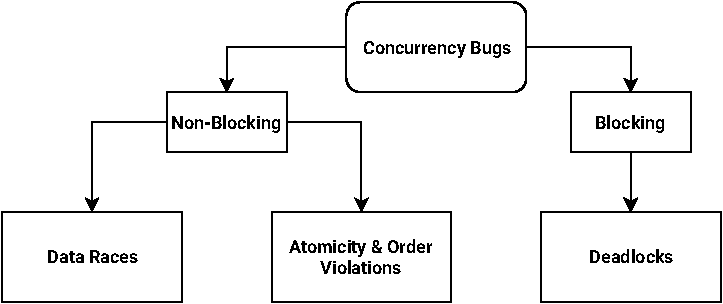
\includegraphics[width=\linewidth]{figures/ConcurrencyBugClasses.pdf}
    \caption{A Taxonomy of Concurrency Bugs -- based on\cite{tchamgoue2012testing}}
    \label{fig:classes}
\end{figure}

\Cref{fig:classes} shows a taxonomy of concurrency bugs based on the work of Tchamgoue, Kim and Jun.~\cite{tchamgoue2012testing}
They distinguish between two main categories of concurrency bugs: \emph{Blocking} and \emph{non-blocking}.
Blocking bugs are bugs where the execution of a program is unintentionally blocked and the program cannot terminate.
% TODO: Meh, don't know if that is right..
The manifestation of these kind of bugs is very noticeable because the whole application freezes and has to be shutdown before the computation can continue.
Non-blocking bugs are often harder to find because they can occur even when the termination of a program was successful but the result is wrong.
This can also lead to a cascade of bugs where the root cause is a non-blocking concurrency bug which might not be obvious.

For example: A method concurrently creates a list of numbers that is expected to be ordered but due to a non-blocking concurrency bug the list suddenly contains unordered elements.
This failure might only occur once in a thousand executions or even less, due to the exponentially growing number of possible thread interleavings.
But if other methods depend on the correct order of the elements in this list, the program might crash or generate wrong results and the reason can be very hard to find.

\subsection{Deadlocks}
\begin{lstlisting}[float=h, language=Go, label=lst:deadlockWG, caption=Deadlock caused by waiting for the \emph{WaitGroup} at a wrong location -- based on \cite{tu2019go}]
func main() {
    var group sync.WaitGroup
    group.Add(len(data))
    for _, d := range data {
        go func(d string) {
            fmt.Printf("Processing: %s\n", d)
            defer group.Done()
        }(d)
        group.Wait() // Causing the bug
    }
}
\end{lstlisting}

The most commonly manifestation of blocking bugs are \emph{deadlocks}, where circular dependencies between resources block the flow of a program.
\Cref{lst:deadlockWG} shows one example of such a deadlock in a Go program.
The problem is a \emph{blocking synchronization} where the \lstinline{group.Wait()} inside the for-loop is causing the block.
This statement has to be moved outside the for loop to resolve the unintentional blocking and fix the concurrency bug.
Although the error seems obvious in this case, those small mistakes can quickly happen and can get unrecognized into the production environment if not tested well enough.

\begin{lstlisting}[float=h, language=Go, label=lst:deadlockCh, caption={Deadlock caused by misuse of an \emph{unbuffered Channel}}]
func main() {
    ch := make(chan int)
    pr := make(chan int)
    ch <- 1 // Program already blocks here
    go func() {
        i := <-ch
        pr <- i
    }()
    <-pr
}
\end{lstlisting}

A second example of a deadlock that might not be obvious is \Cref{lst:deadlockCh} which uses two unbuffered channels to transfer information between threads.
The problem here is that without an active listener on an unbuffered channel, any send action will be blocked.
To fix this, one could replace the unbuffered channel with a buffered one, so that the execution flow of the program can continue without blocking.
This shows how important it is to know the concrete implementation of a concurrency abstraction.
Even though intended to ease the synchronization between threads and make inter-thread communication safer, by not knowing the implementation of an abstraction the developer can unknowingly create hard to find concurrency bugs.

Another common problem in event-driven concurrent programs are \emph{blocking operations} like filesystem operations that are executed inside an event-handler.
These ``can penalize and even paralyze the entire program execution.''~\cite{tchamgoue2012testing}

\subsection{Data Races}
\begin{lstlisting}[float=h, language=Go, label=lst:race, caption=Data race -- based on \cite{goRaceDetector}]
func main() {
	c := make(chan bool)
	m := make(map[string]string)
	go func() {
		m["1"] = "a" // First conflicting access.
		c <- true
	}()
	m["2"] = "b" // Second conflicting access.
	<-c
}
\end{lstlisting}

Data races are part of the non-blocking concurrency bugs.
They occur when multiple threads simultaneously try to access a shared variable where at least one access is a write operation.~\cite{serebry2009threadsanitizer}

\Cref{lst:race} shows an example of a data race that is frequently found.~\cite{serebry2009threadsanitizer}
The data race happens when ``two threads access a non-thread-safe complex object [e.g. a map] without synchronization.''~\cite{serebry2009threadsanitizer}
Even though the two threads in this example write to different keys of the map \lstinline{m}, this might cause a corruption of data or even crash the program because the default Go map implementation is not concurrency-aware.
To fix this, the access to the map needs to be synchronized by a lock for example.

% TODO: Is it a data race or an atomicity violation?
A special case of data races are multi-variable data races.
In this case multiple variables that are semantically correlated are accessed by multiple threads and could therefore loose their semantic correctness when not handled correctly.
A common example for this are structs that have a data and a length field.
Whenever the data field gets updated, so does the length field which is semantically correlated with the data.
When multiple threads update these variables they need to synchronize not only on each of the variables separately but on all semantically correlated variables at the same time.~\cite{lu2007muvi}

\subsection{Atomicity and Order Violations}
\begin{lstlisting}[float=h, language=Go, label=lst:order, caption=Test-and-Use bug pattern -- Order violation]
func main() {
    data := getData()
    go func() {
        process(data)
        data = nil
    }()
    if (data != nil) {
        process(data) // Might already be nil
    }
}
\end{lstlisting}

Atomicity and order violations are concurrency bugs where the interleaving of threads violate the programmer's intention of atomicity and order.
This often happens because:
``Most programmers think sequentially and therefore they make mistakes easily when writing concurrent programs.''~\cite{lu2008mistakes}

\Cref{lst:order} shows a common order violation bug pattern called ``Test-and-Use''.
The programmer's intention is to check if a variable is not \lstinline{nil} and then use this variable.
However, due to the thread that was launched before, it could happen that after the \lstinline{if} check in line 7, the thread of the goroutine gets scheduled and the data variable is set to \lstinline{nil}.
To fix this bug, the check and the usage of the variable need to become an atomic operation to enforce the order of execution.

\begin{lstlisting}[float=h, language=Go, label=lst:atomicity, caption=Load-Store bug pattern -- Atomicity violation]
func main() {
    var group sync.WaitGroup
    group.Add(10)
    sum := 0
    for i = 0; i < 10; i++ {
        go func() {
            defer group.Done()
            sum++ // Not atomic
        }()
    }
    group.Wait()
}
\end{lstlisting}

\Cref{lst:atomicity} shows one example of the infamous ``Load-Store'' bug pattern.
The programmer assumes that ++ is an atomic operation because it is one literal in Go.
However, after compilation this is expanded to 3 instructions: LOAD, INCREMENT and finally STORE.
The thread scheduler could switch the context after any of these instructions what leads to undefined behavior, when multiple threads try to increment the same variable.
To fix this bug pattern, the \lstinline{++} operation also needs to be replaced by an atomic operation that does not allow other threads to access the \lstinline{sum} variable while incrementing.

Lu, Park, Seo and Zhou conducted a study in 2008 where they analyzed the characteristics of real-world concurrency bugs.~\cite{lu2008mistakes}
One key finding was that:
``Most of the examined non-deadlock concurrency bugs are covered by two simple patterns: atomicity-violation and order-violation''~\cite{lu2008mistakes}

A promising solution to atomicity and order violation bugs is \emph{software transactional memory} (STM) as proposed by Peyton Jones.~\cite{peytonjones2007beautiful}
It is an alternative to traditional lock-based synchronization where atomic regions get declared explicitly.
Languages like Haskell provide STM by their design of language but Go can also utilize this mechanism by using external libraries.

% ------------------------------------ %
% ------ DYNAMIC CODE ANALYSIS ------- %
% ------------------------------------ %
\section{Dynamic Code Analysis}
\label{sct:dynamic}

One of the main techniques for finding concurrency bugs is dynamic code analysis.
% TODO: Find better word for problematic
In dynamic code analysis the runtime behavior of a program is observed to detect problematic patterns like unsynchronized variable accesses or deadlocks.

One popular implementation of this is ``Record and Replay'' where the path of execution of an application is recorded and can later be deterministically replayed.
This way developers can easily find and fix those bug because, ``detecting concurrency bugs is difficult but once detected; correcting them is somehow an easy job.''~\cite{tchamgoue2012testing}
To create a recording that contains all information to replay a program exactly the same way it was executed, the recorder needs to keep track of the schedule of the program as well as all variables that might not be deterministically reproducible.
Furthermore, any source of non-determinism such as the the interaction with the network or graphics card or any call to external libraries need to be recorded.~\cite{lidbury2019sparse}
Like expected, this creates a lot of computational overhead in CPU time as well as storage.
This approach also forms the foundation for many other techniques and has many different variants and implementations.

To track the schedule of a natively compiled program such as Go programs, the record tool has to sit between the host operating system and the application.
One requirement to use such a tool in production is the ease of deployability which means that the operational overhead should be very small.
There have been approaches with custom hardware or patched operating system kernels to hijack the scheduler, but these setups are quite complex and not easy to deploy.
One example for a tool that fulfills this requirement is \emph{rr}~\footnote{\url{https://rr-project.org/}} developed by \emph{Mozilla}.
Their approach is to run the program to observe on a fixed CPU core and track the system calls by using \emph{\_ptrace\_}.
This way they can record programs on an unmodified Linux system and without compiling instrumentation into the programs code which might affect the concurrency behavior.
The main performance bottleneck beside the execution on only one CPU core, are the context switches induced by ptrace.~\cite{o2017engineering}
Lidbury and Donaldson~\cite{lidbury2019sparse} examined further ways to reduce the computational overhead by a sparse recording approach.
By selectively ignoring ``unimportant'' sources of non-determinism they were able to record input and output heavy applications like video games with an acceptable overhead where as \emph{rr} was not able to record at all due to the massive overhead of recording every source of non-determinism.
During replay they execute the thread schedule as recorded and mock every source of recorded non-determinism but let the ignored regions of the program execute non-deterministically.

Record and replay could therefore be a great tool to monitor applications in production.
Once a bug occurs and is either reported by a user or by the program itself, the programmer could just replay the thread schedule to reproduce, find and therefore fix the bug quickly.
Additionally, this technique can help to reproduce all kind of concurrency bugs, no matter if they are blocking or non-blocking.
For programs that do not heavily depend on parallelism this approach is also very feasible.
The tool \emph{rr} can record such programs with a performance overhead below the factor of two.
However, for programs that heavily rely on parallelism the overhead to record and store the thread schedule and all necessary parameters can decrease the performance by more than a factor of 30.~\cite{o2017engineering}
Especially for multi-threaded server applications that expect a high workload and where speed is crucial for the business, this approach is not feasible in production, yet.
And even if the workload is low but the application is time-sensitive for example because of protocol timeouts, it is not applicable without extending the acceptable timeouts.

Another set of tools for dynamic code analysis are dynamic data race detectors.
As the name implies, these tools detect data races but because atomicity and order violations are often correlated, these tools can detect a variety of non-blocking concurrency bugs.
There are multiple approaches for data race detection but in this case we refer to on-the-fly and post-mortem data race detection which are often referred to as dynamic.~\cite{serebry2009threadsanitizer}
One data race detector that is mainly used for Go programs is the \emph{ThreadSanitizer} developed by Google.
It is built in the Golang compiler tool-chain and can be toggled with a simple compiler flag which makes it very easy to use.
``The tool performs compile-time instrumentation of the source program, in which all (atomic and non-atomic) accesses to potentially shared locations, as well as fence operations, are instrumented with calls into a statically linked run-time library.''~\cite{lidbury2019sparse}
To distinguish between synchronized accesses and data races during runtime, the compiler also has to inject dynamic annotations into the program.
With these annotations the data race detector understands the synchronization primitives used by the programming language.
When the program along with the race detector gets executed, the data race detector ``observes the program execution as a sequence of events.''~\cite{serebry2009threadsanitizer}
To detect a data race, there are two algorithms that are mainly used among all detectors: \emph{happens-before} and \emph{lockset}.
Locking events are Write and Read Locks / Unlocks.
Happens-before events are Signal and Wait.
The \emph{ThreadSanitizer} uses an hybrid approach by combining both algorithms into one and observing events of both categories.

Performance-wise the race detection is unfortunately not better than the record and replay approach.
The official race detector article on the Go website claims: ``The cost of race detection varies by program, but for a typical program, memory usage may increase by 5-10x and execution time by 2-20x.''~\cite{goRaceDetector}
Which is in fact better than the original 20x-50x evaluated by Serebryany and Iskhodzhanov in 2009.~\cite{serebry2009threadsanitizer}
However, a possible improvement could be to ignore certain uncritical regions and just observe hotspots where data races are suspected.


Beside their ease of use, one of the main disadvantages of dynamic analysis tools is their coverage, that `` [...] is typically small since only a few executions are explored.''~\cite{qadeer2004kiss}
Additionally, they depend on the manifestation and especially the recognition of these bugs to report them correctly.


% ------------------------------------ %
% ---- CONCURRENCY-AWARE TESTING ----- %
% ------------------------------------ %
\section{Concurrency-aware Testing}
\label{sct:testing}

\begin{figure}
    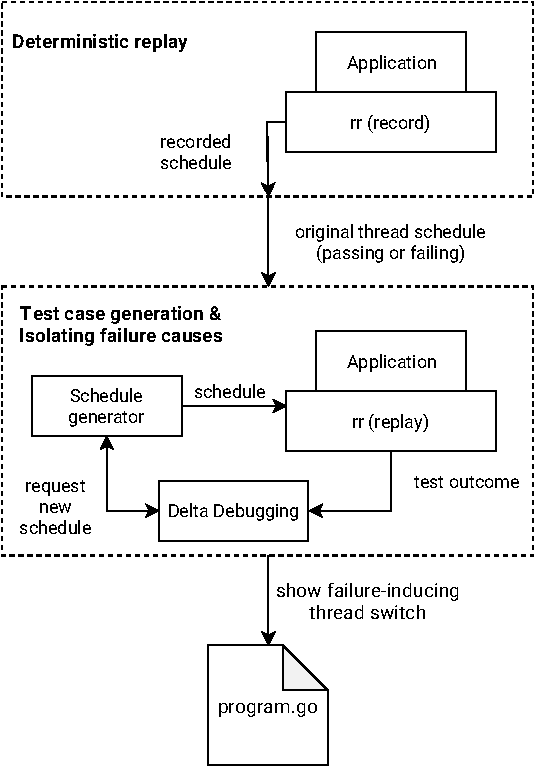
\includegraphics[width=\linewidth]{figures/Concurrency-Testing.pdf}
    \caption{Automatic concurrency-aware testing for Go programs -- based on\cite{acm2002}}
    \label{fig:testing}
\end{figure}

Extensive testing has proven to minimize the bugs of software in production.\cite{makinen2014testing}
However, traditional testing mostly covers sequential errors and cannot detect concurrency bugs effectively.\cite{lu2008mistakes}
This lies in the nature of these bugs themself.
When only certain thread interleavings trigger the bug, the tests could complete successfully almost every time without ever finding a manifestation.
So, new concurrency-aware tests are needed to find concurrency bugs reliably.

One early attempt to test programs for concurrency bugs was to inject delays at random points in the program code, but it is yet unclear if this really gives an acceptable bug coverage.~\cite{lu2008mistakes}
Furthermore, the tests should try to reduce the perturbation on the execution, so the software can be evaluated the same way as it would run in a regular deployment in production.

Another method of concurrency-aware testing has been proposed by Choi and Zeller.\cite{acm2002}
They implemented a tool called ``DEJAVU'' for the \emph{Jalapeño} Java Virtual Machine but the concept is also applicable to tools that work with Go or any other programming language.
They make use of a technique called \emph{Delta debugging}, which describes the process of narrowing down the spot where a failure is introduced by going back and forth between working and non-working conditions, in this case working and non-working thread schedules.~\cite{zeller2002delta}
\Cref{fig:testing} shows a modified model of the \emph{DEJAVU} approach, suited for Go programs by using rr instead of of \emph{DEJAVU} for the recording and replay of the thread schedule.
As a prerequisite, test cases need to be created that define the expected behavior of the application.
These can either succeed or fail which can be shown by the exit code for example.
In the first step, the Go application with these test cases gets executed and the thread schedule gets recorded by \emph{rr}.
The either failing or succeeding recorded thread schedule is then passed to the next instance where the delta debugging unit requests new executions of the application with an alternated thread schedule until it can pinpoint the failure-inducing thread switch.
The thread schedule is generated by the \emph{Schedule generator} and is replayed by the replay module in \emph{rr}.
The schedule as well as the test result is passed back to the delta debugging unit.
``By systematically narrowing down the difference between a thread schedule that makes the program pass and another schedule that makes the program fail, the Delta Debugging approach can pinpoint the error location automatically -- namely the location(s) where a thread switch causes the program to fail.''~\cite{acm2002}

While this technique cannot be used in a productive deployment setup, it is intended to extend existing tests that for example run inside a CI pipeline.
One major drawback however, is the number of thread interleavings that can grow exponentially with the number of executed threads.
But for most cases it is not necessary to evaluate all possible thread schedules.
Lu et al. have found in their study of real-world concurrency bugs that ``Almost 96\% of the examined concurrency bugs are guaranteed to manifest if certain partial order between 2 threads is enforced.''~\cite{lu2008mistakes}
Which means that ``Pairwise testing on concurrent program threads can expose most concurrency bugs, and greatly reduce the testing complexity.''~\cite{lu2008mistakes}
To increase the coverage of concurrency bugs, this approach could also be combined with a data race detector to dynamically detect data races within certain replays of a thread schedule.
This way the test cases can be minimized to semantical correctness checks, which decreases the operational overhead for such a setup.
The setup of such a system also comes with a relatively low operational overhead because once such a system is build, it could be easily embedded within the CI pipelines of a project.


% ------------------------------------ %
% ------ STATIC CODE ANALYSIS -------- %
% ------------------------------------ %
\section{Static Code Analysis}
\label{sct:static}

Static code analysis describes the technique of predicting the behavior of a program by analyzing the source code without compiling nor executing it.

A common approach to static code analysis is model-checking where the code gets translated into mathematical models such as state machines or graphs.
But model checking for concurrent programs is complex due to the number of possible thread interleavings that can grow exponentially with the number of executed threads.
Therefore, static data race detectors for example are unfeasible for very large code bases.~\cite{serebry2009threadsanitizer}

One implementation of static code analysis to detect concurrency bugs is sequentialization as proposed by Qadeer and Wu.~\cite{qadeer2004kiss}
Their approach is to transform a parallel program into a sequential one and simulate a large subset of the behavior of the parallel program on the sequential one.
This way they can use traditional and highly optimized sequential model-checkers to analyze the application.
By this approach the system has no false-positive reports on concurrency bugs but the overall coverage is not very high.

Although unfeasible for detecting data races in large code bases, there are multiple implementations of static deadlock-detectors for concurrent programs.
One concrete static deadlock detector for the Go programming language is called \emph{Godel Checker}.~\cite{godelChecker}
It uses that Go's message passing concurrency mechanisms by channels is ``[...] greatly inspired by advances in formal languages for concurrency theory known as process calculi.''~\cite{lange2018verification}
The \emph{Godel Checker} tool extracts the main concurrency characteristics of the program into a mathematical model called \emph{Behavioural Types}.
These types can be further processed into a \emph{static single assignment}, which then can be processed by classical model and termination checker.
This way not only total deadlocks where all threads are stuck, but also partial deadlocks and channel safety threats can be found.

The computational overhead for this approach is also surprisingly low.
A program with 18 kLOC can be checked within minutes.~\cite{lange2018verification}
Unfortunately this technique has quite a few limitations.
Only immutable Go channels are supported that are not located in a dynamic data type.
Furthermore, Go does not force the developer to use synchronization by message passing, so any deadlocks introduced by traditional locking mechanisms will be not be noticed.


% ------------------------------------ %
% ------------ CONCLUSION ------------ %
% ------------------------------------ %
\section{Conclusion}
\label{sct:conclusion}

While having multi-threaded applications is convenient and also necessary in today's world of computation, the non-determinism makes it hard to find, reproduce and therefore fix concurrency bugs.
Although there is a variety of tools that try to ease the process of multi-threaded debugging, as shown, none of them really fulfills all requirements for a production-ready drop-in solution.

Dynamic code analysis has the main disadvantage that it can cost a lot of overhead when monitoring is active in a production environment.
Especially programs that heavily rely on multi-threaded execution like web-servers  can become very inefficient or could even fail due to timeout limitations.
Dynamic data race detectors could eventually be optimized to an acceptable overhead by ignoring most of the assumed-to-be-safe code regions, but this also drastically lowers the overall coverage.
Beside that, ``data-race free does not mean concurrency bug free.''~\cite{lu2008mistakes}
The main advantage of the dynamic approach is that it theoretically could be deployed to a real production environment.
For programs that are mainly event-driven this would give the ability to observe the real-world behavior in a reproducible way.

Concurrency-aware testing is very promising in the regard of extending an existing testing pipeline.
This way concurrency bugs could be detected even before the software is deployed into production.
The overhead can be minimized by optimizing the thread schedule generator and by ignoring most uncritical regions of the code.
However, the coverage depends on the quality of the tests that also need to be aware of multi-variable semantic data races.

Static code analysis is only feasible in small code bases, due to the exponentially growing thread interleavings that need to be explored, which requires a lot of computational overhead.
Additionally multi-variable accesses of only semantically correlated variables need manual annotations or configuration.
``Unfortunately, existing techniques cannot effectively extract such semantic correlations. Traditional compiler analysis cannot catch them, because many correlated variables are just semantically correlated and do not necessarily have data dependencies, [...]''~\cite{lu2007muvi}
Beside that there are some promising tools for statically finding deadlocks by translating programs into a mathematical model.

Concluding this paper, the evaluation of the different approaches shows that there is not one tool to solve all problems that arise when writing concurrent programs.
But there are multiple techniques that can be combined to at least get some support in debugging multi-threaded applications.

However, for modern micro-service architectures that get more and more popular, these tools could actually be useful because the code bases tend to get smaller.
That means that the overhead of instrumenting, testing or model-checking these applications gets smaller in absolute numbers.
Record and replay could also be deployed to just some replicas of an instance, reducing the impact on crucial business speed whilst collecting useful information to optimize the whole code base.

But then again, detecting and reporting concurrency bugs is just the first step in fixing them.
Developers need to understand the reporting and need to distinguish between real bugs and false-positives.
So, ``There is no silver bullet for fixing concurrency bugs.''~\cite{lu2008mistakes}


\bibliographystyle{IEEEtran}
\bibliography{references}

\end{document}
